\documentclass[10.5pt,a4paper]{article}
\usepackage[margin=1.9cm]{geometry}
\usepackage{amsmath,array,graphicx,booktabs,xurl,hyperref,enumitem,float,caption,listings,xcolor,tabularx}
\hypersetup{colorlinks=true,urlcolor=blue,linkcolor=black}
\setlist{itemsep=1pt,topsep=3pt}
\captionsetup{font=small,labelfont=bf}
\lstset{basicstyle=\ttfamily\footnotesize,frame=single,breaklines=true,columns=fullflexible,backgroundcolor=\color{gray!6}}
\setlength{\parskip}{4pt}\setlength{\parindent}{0pt}
\title{\textbf{Lab 8: OpenTelemetry for the Village Pond Planning System}}
\author{Sneha Nagmoti \\ \small Indian Institute of Technology Bhilai \quad \texttt{snehan@iitbhilai.ac.in}}
\date{16 October 2026}
\begin{document}
\sloppy
\maketitle

\section{Overview}
OpenTelemetry (OTel) was added to my Assignment~1 backend (FastAPI service \texttt{village-pond-api}). The service now emits all three signals over OTLP: \textbf{traces} (one per request, with a child span for every external data source and every terrain/hydrology stage), \textbf{metrics} (request counts, latency, per-stage time, catchment area, runoff volume, external-source failures) and \textbf{logs} (every Python log record, tagged with the trace and span that produced it). An OpenTelemetry Collector routes traces to \textbf{Jaeger}, metrics to \textbf{Prometheus}, and logs to a JSON file and its console. All screenshots below were taken from my own running project processing the supplied \texttt{contours\_1m.kml}.

Code: \url{https://github.com/snehanagmoti/Village-Pond-planning} (commits \texttt{bacc3d2}, \texttt{2365037}; files \texttt{backend/observability.py}, \texttt{observability/}).

\section{Implementation}
\subsection{Architecture}
\begin{center}
\small
\texttt{FastAPI app (OTel SDK)} $\xrightarrow{\text{OTLP/HTTP :4318}}$ \texttt{OTel Collector} $\rightarrow$
\begin{tabular}{l}
\texttt{traces} $\rightarrow$ Jaeger (UI :16686)\\
\texttt{metrics} $\rightarrow$ Prometheus exporter :8889 $\leftarrow$ scraped by Prometheus (UI :9090)\\
\texttt{logs} $\rightarrow$ \texttt{logs.jsonl} file + debug console
\end{tabular}
\end{center}
Sending everything to a Collector (instead of directly to Jaeger/Prometheus) keeps the application vendor-neutral: changing a backend only changes \texttt{collector.yaml}, not the code.

\subsection{What is instrumented}
\textbf{Setup (\texttt{backend/observability.py}).} \texttt{setup\_observability(app)} creates a \texttt{Resource} (\texttt{service.name=village-pond-api}, \texttt{service.version}, \texttt{deployment.environment}), a \texttt{TracerProvider} with a \texttt{BatchSpanProcessor}, a \texttt{MeterProvider} with a 5-second \texttt{PeriodicExportingMetricReader}, and a \texttt{LoggerProvider} with a \texttt{BatchLogRecordProcessor}, all using OTLP/HTTP exporters. Telemetry is \emph{opt-in} (\texttt{OTEL\_ENABLED=true}). When disabled, or if the packages are missing (e.g.\ on the older lab deployment), every helper is a no-op, so behaviour is unchanged. 87 backend tests pass, including a new test that checks the pipeline spans and metrics with an in-memory exporter.

\textbf{Automatic instrumentation.} \texttt{FastAPIInstrumentor} creates a server span per request (method, route, status code, client) and the standard \texttt{http.server.*} metrics. \texttt{HTTPXClientInstrumentor} creates a client span for every outgoing call to the elevation, imagery, map-tile and rainfall APIs, so failures of third-party services appear inside the request trace.

\textbf{Manual spans} (with a context-manager helper \texttt{span(name, **attributes)}):
\begin{center}\small
\begin{tabularx}{\linewidth}{@{}>{\raggedright\arraybackslash}p{6.4cm}X@{}}\toprule
Span & Attributes recorded\\\midrule
\texttt{external.satellite\_imagery}, \texttt{external.mapped\_hydrography}, \texttt{external.rainfall}, \texttt{external.elevation} & error status + exception when a source fails\\
\texttt{contour.parse\_kml} & file size, file name, number of contour lines\\
\texttt{terrain.harmonic\_interpolation} & grid rows/columns, cell size, iterations, converged\\
\texttt{water.exclusion\_mask} & detected-water ratio, excluded cells (60 m buffer)\\
\texttt{terrain.priority\_flood} & filled cells, maximum fill depth\\
\texttt{terrain.resolve\_flats\_d8}, \texttt{terrain.flow\_accumulation} & maximum accumulation\\
\texttt{terrain.rank\_candidates} & eligible cells, selection mode, options ranked\\
\texttt{terrain.delineate\_catchment} & catchment cells and hectares\\
server span (result) & \texttt{pond.catchment\_ha}, \texttt{pond.runoff\_m3}, \texttt{pond.capacity\_m3}, \texttt{pond.selection\_mode}, \texttt{pond.analysis\_status}, pond coordinates\\\bottomrule
\end{tabularx}\end{center}
The CPU-heavy pipeline runs in a worker thread (\texttt{asyncio.to\_thread}); because that call copies the context, the stage spans are correctly nested under the request span.

\textbf{Custom metrics:} \texttt{pond.analysis.requests} (counter: workflow, HTTP status, outcome), \texttt{pond.analysis.duration} and \texttt{pond.pipeline.stage.duration} (histograms, seconds), \texttt{pond.catchment.area} (ha) and \texttt{pond.runoff.volume} (m\textsuperscript{3}) histograms, and \texttt{pond.external\_source.failures} (counter: source, reason). Default OTel histogram buckets are designed for milliseconds; with them the p95 of a 1.3~s analysis was reported as 4.75~s, so explicit second-scale bucket boundaries were configured.

\textbf{Logs:} an OTel \texttt{LoggingHandler} on the root logger exports every record with its trace/span id; a logging filter also prints \texttt{[trace\_id=… span\_id=…]} on console lines. New log events record each completed analysis and every external-source failure.

\subsection{Tools, libraries and backend services}
\begin{center}\small
\begin{tabular}{@{}ll@{}}\toprule
Component & Version / role\\\midrule
\texttt{opentelemetry-api}, \texttt{-sdk}, \texttt{-exporter-otlp-proto-http} & 1.45.1 — providers, processors, OTLP/HTTP exporters\\
\texttt{opentelemetry-instrumentation-fastapi}, \texttt{-httpx} & 0.66b1 — automatic server and HTTP-client spans\\
OpenTelemetry Collector (contrib) & 0.111.0 — OTLP receiver; Jaeger, Prometheus, file and debug exporters\\
Jaeger all-in-one & 1.62.0 — trace storage and UI\\
Prometheus & 2.53.2 — metric scraping, PromQL and UI\\
Application & FastAPI, Uvicorn, NumPy, OpenCV (Assignment 1 code)\\\bottomrule
\end{tabular}\end{center}

\subsection{How it was run}
Two instances of the same app were started with \texttt{observability/run\_app.py}. They are distinguished by the resource attribute \texttt{deployment.environment}:
\begin{itemize}
\item \textbf{\texttt{lab-live-network}} (port 8002) uses the real external adapters. My lab machine has no access to the Esri/OpenStreetMap tile servers or the rainfall and elevation APIs, so these requests show genuine failures.
\item \textbf{\texttt{lab-offline-fixtures}} (port 8001) replaces \emph{only} the three external data adapters (satellite tiles, OSM tiles, rainfall) with deterministic local fixtures: no water detected, and about 1,216 mm/year of rain. KML parsing, interpolation, Priority-Flood, D8, ranking, catchment and runoff code run unchanged on the real \texttt{contours\_1m.kml}. Because the fixture detects no water, the catchment numbers (50.32 ha) differ slightly from the deployed site (50.90 ha).
\end{itemize}
Workload sent with \texttt{curl}: automatic, point and region contour analyses (HTTP 200); a point on the river, a missing upload, a wrong field name and a malformed KML (HTTP 422); a burst that hit the rate limit (HTTP 429); contour and live analyses on the network instance (HTTP 503); and health checks.

\section{Screenshots and what they show}

\begin{figure}[H]\centering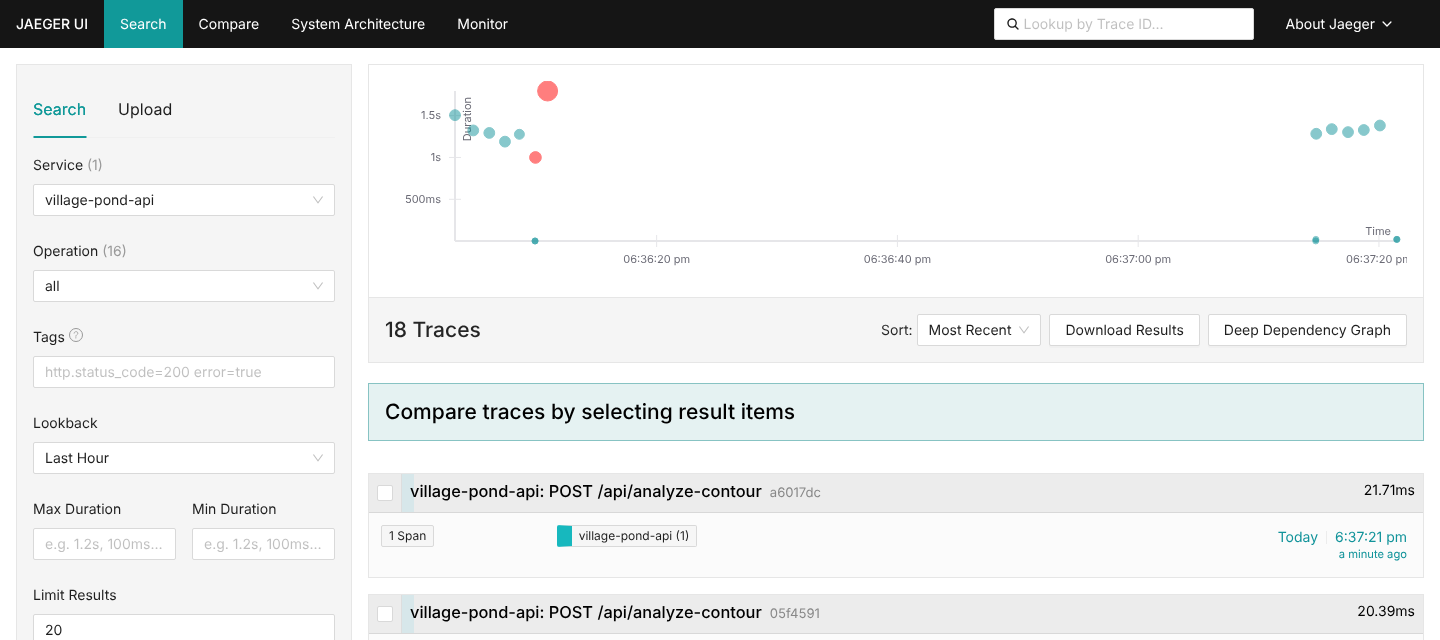
\includegraphics[width=\linewidth]{figures/f1_jaeger_search.png}
\caption{Jaeger search for service \texttt{village-pond-api}. Each dot/row is one request trace; the y-axis is duration. Successful contour analyses take about 1.3--1.5 s with 12 spans, rejected requests (422/429) take milliseconds with 1 span, and failed requests (503) show error markers.}\end{figure}

\begin{figure}[H]\centering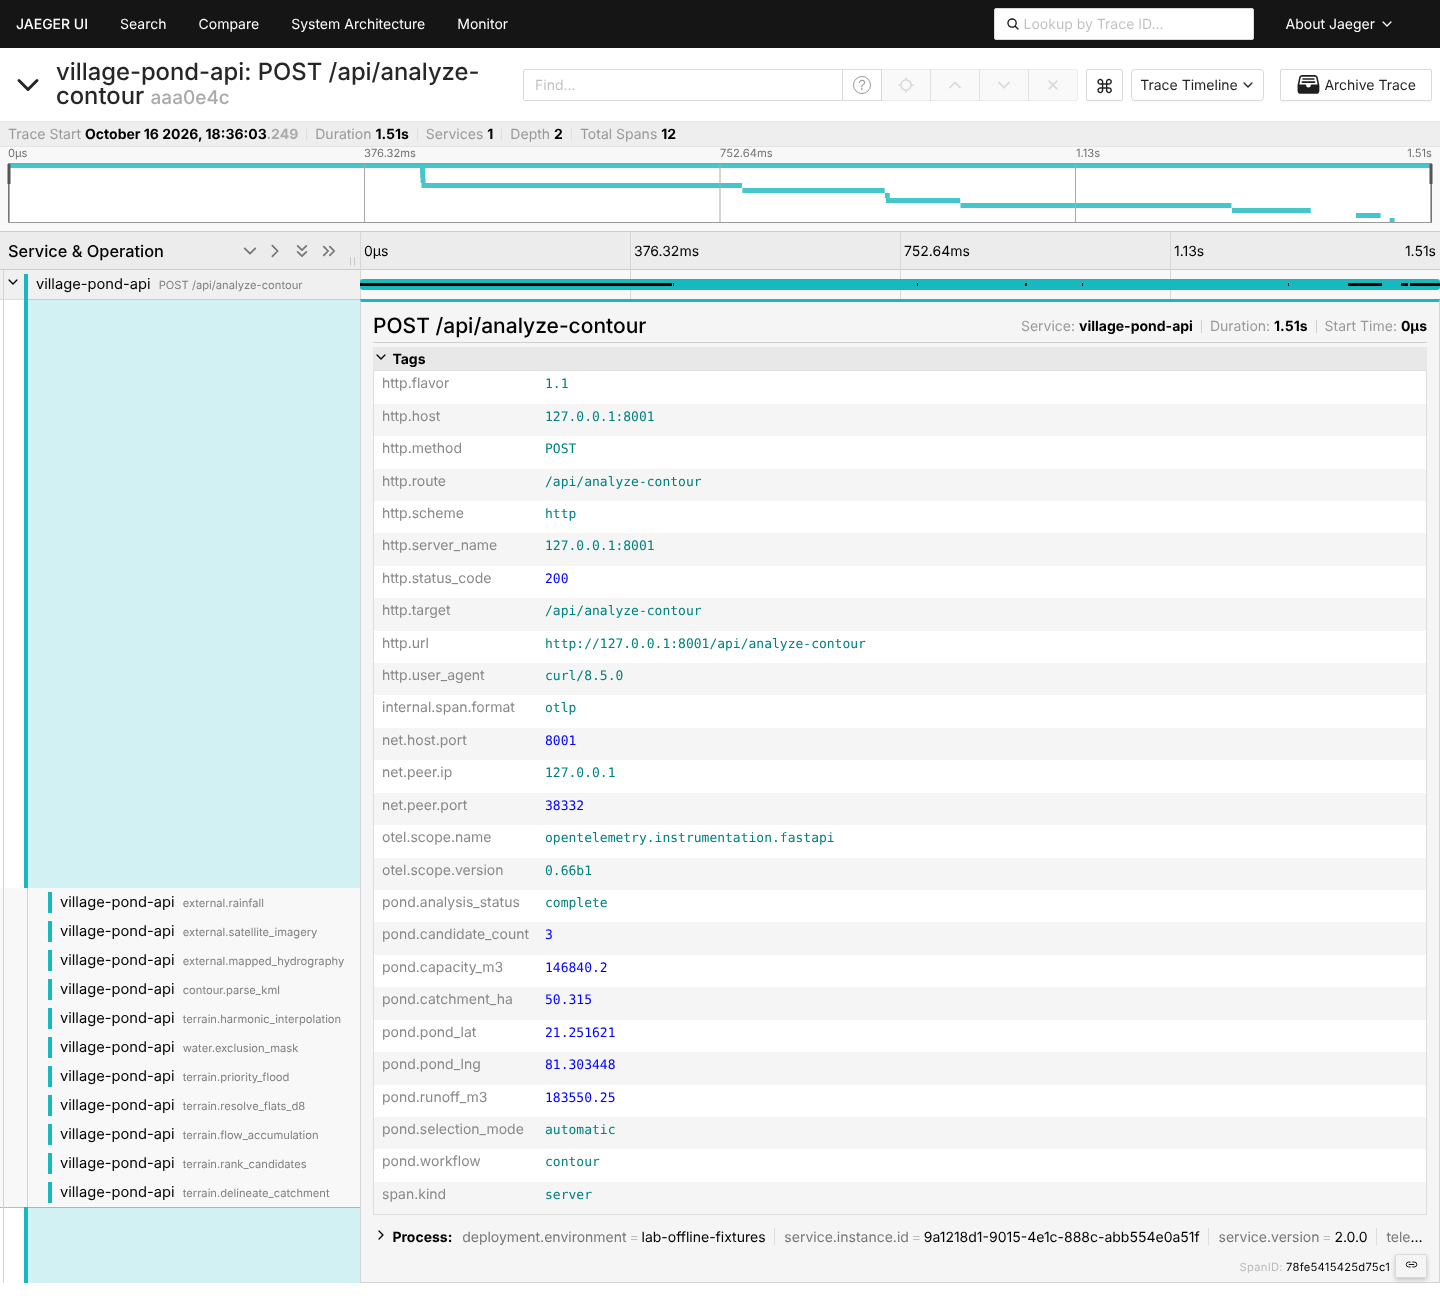
\includegraphics[width=0.93\linewidth]{figures/f2_trace_success.png}
\caption{Trace of one successful automatic contour analysis (1.51 s, 12 spans). The waterfall shows the three external fetches running \emph{in parallel} (asyncio.gather), then KML parsing (339 ms), harmonic interpolation (150 ms), water exclusion (1 ms), Priority-Flood (77 ms), flat resolution + D8 (286 ms), flow accumulation (63 ms), ranking (26 ms) and catchment delineation (3 ms). The server-span tags carry the scientific result: catchment 50.315 ha, runoff 183,550 m\textsuperscript{3}/year, capacity 146,840 m\textsuperscript{3}, pond at 21.251621, 81.303448, 3 candidates, mode \texttt{automatic}.}\end{figure}

\begin{figure}[H]\centering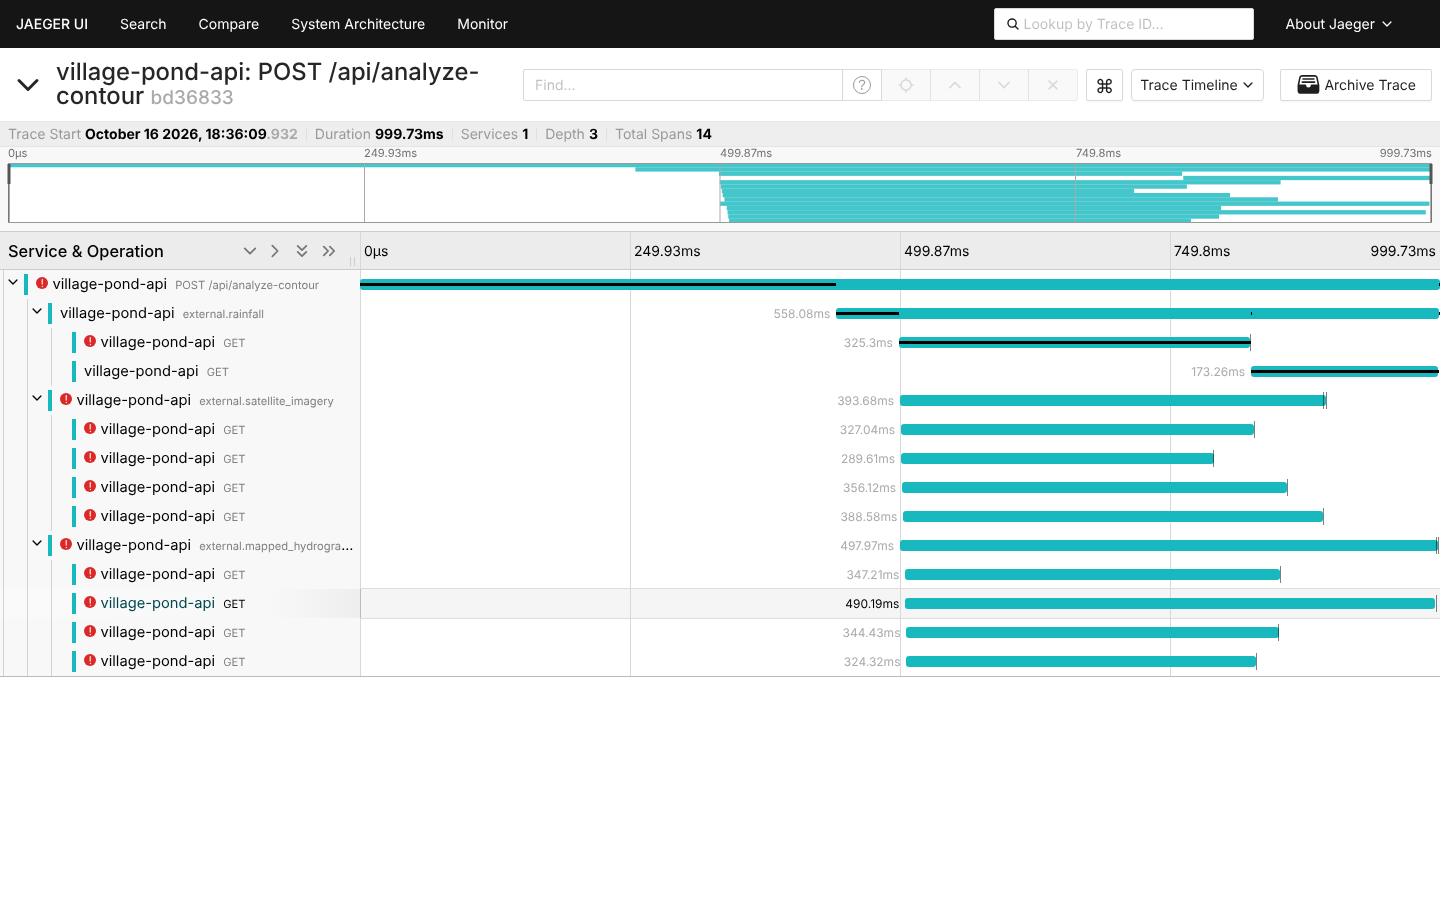
\includegraphics[width=\linewidth]{figures/f3_trace_failure.png}
\caption{Trace of a contour request on the \texttt{lab-live-network} instance that returned HTTP 503. Red error icons mark the failed spans. Under \texttt{external.satellite\_imagery} and \texttt{external.mapped\_hydrography}, the auto-instrumented httpx \texttt{GET} spans show each tile download failing. The request fails closed: no pond is recommended without water screening.}\end{figure}

\begin{figure}[H]\centering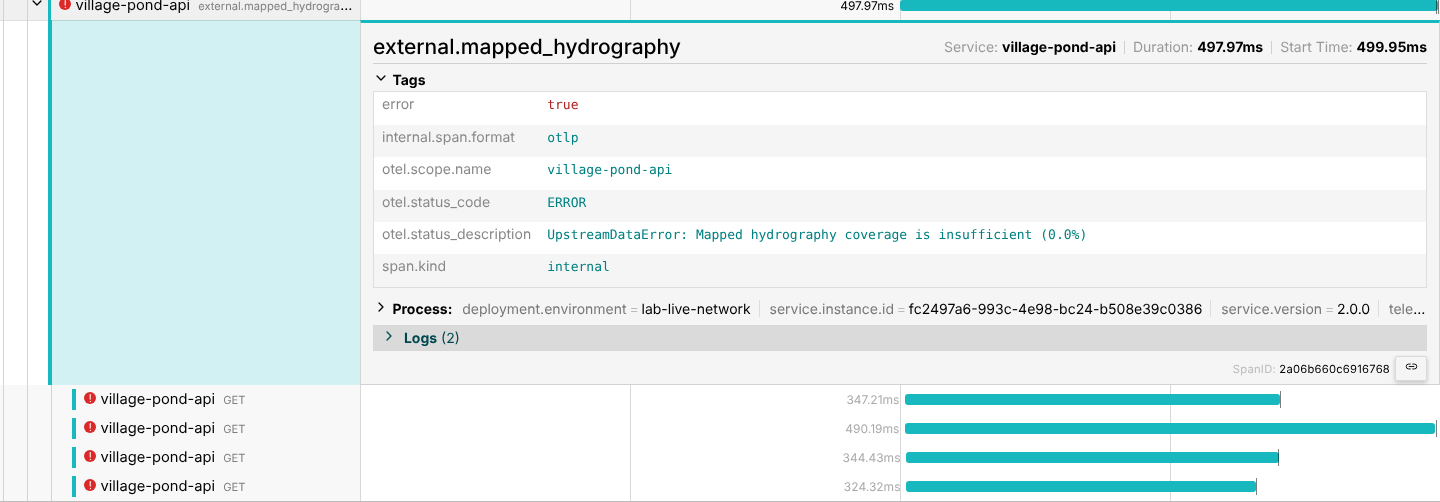
\includegraphics[width=\linewidth]{figures/f4_span_failure.png}
\caption{Detail of the failed \texttt{external.mapped\_hydrography} span: \texttt{error=true}, \texttt{otel.status\_code=ERROR} and the exact reason \emph{``Mapped hydrography coverage is insufficient (0.0\%)''}. The \texttt{Process} line shows the resource attributes identifying which deployment produced the span.}\end{figure}

\begin{figure}[H]\centering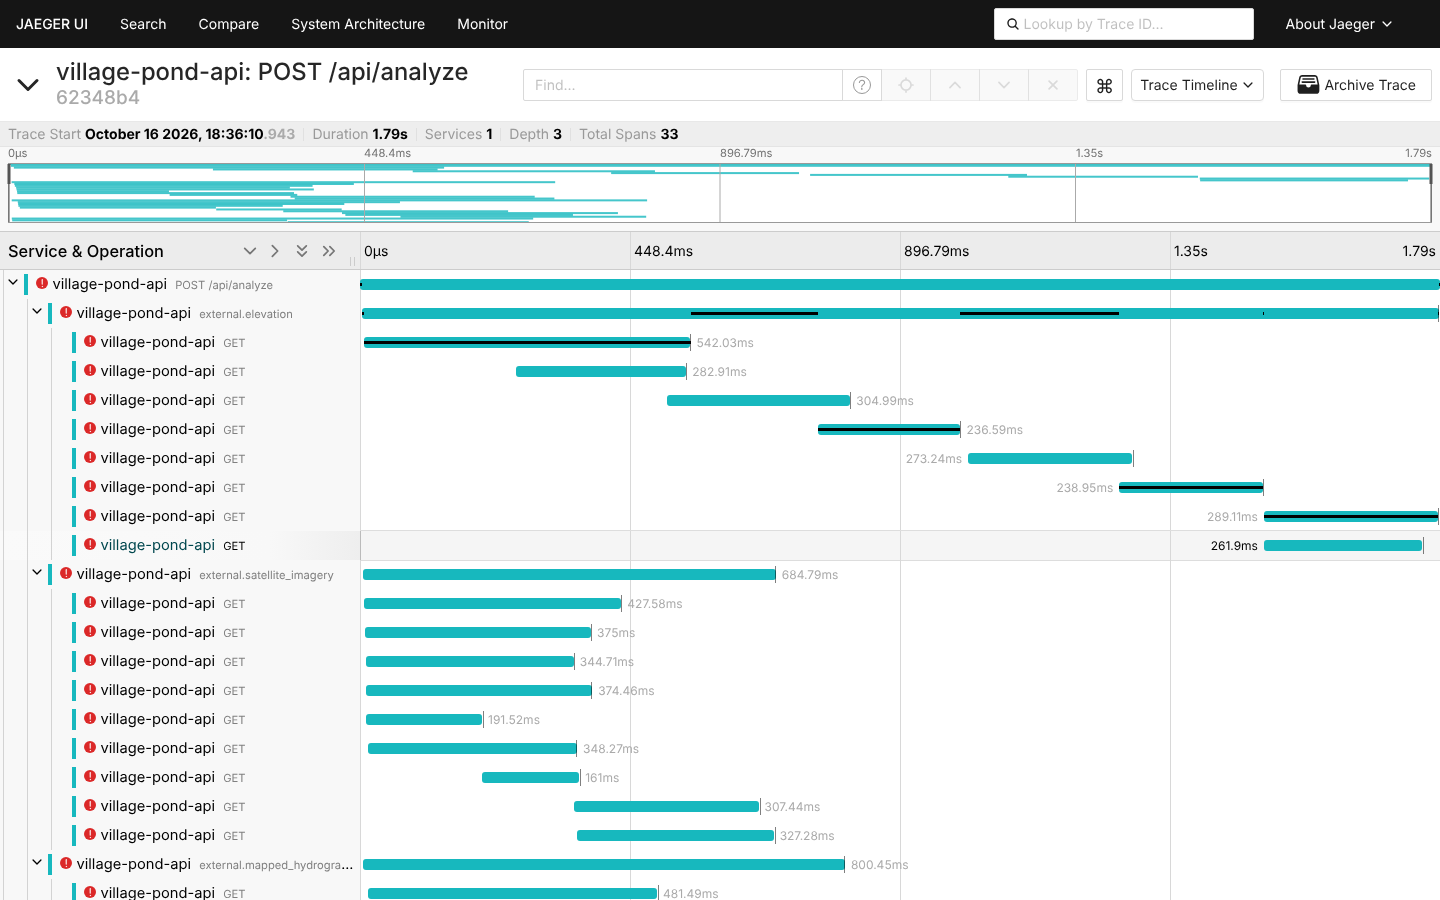
\includegraphics[width=\linewidth]{figures/f5_trace_live_failure.png}
\caption{Live-map analysis (\texttt{POST /api/analyze}, 33 spans, 1.79 s) failing with 503. The elevation adapter tries six batch requests and then its tile fallback; every attempt is a separate red \texttt{GET} span. The trace shows where the 1.8 s went (retries against an unreachable service), which a single error message could not.}\end{figure}

\begin{figure}[H]\centering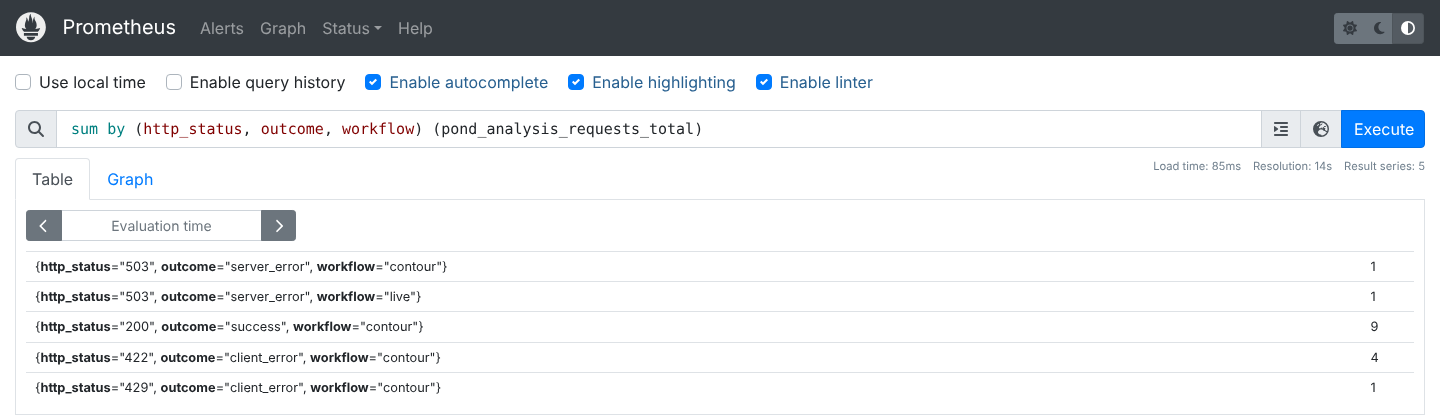
\includegraphics[width=\linewidth]{figures/f6_prom_requests.png}
\caption{Prometheus: \texttt{pond.analysis.requests} by HTTP status, outcome and workflow (9 successes, 4 validation errors, 1 rate-limited request, 2 upstream failures). This is the error-rate view used for monitoring.}\end{figure}

\begin{figure}[H]\centering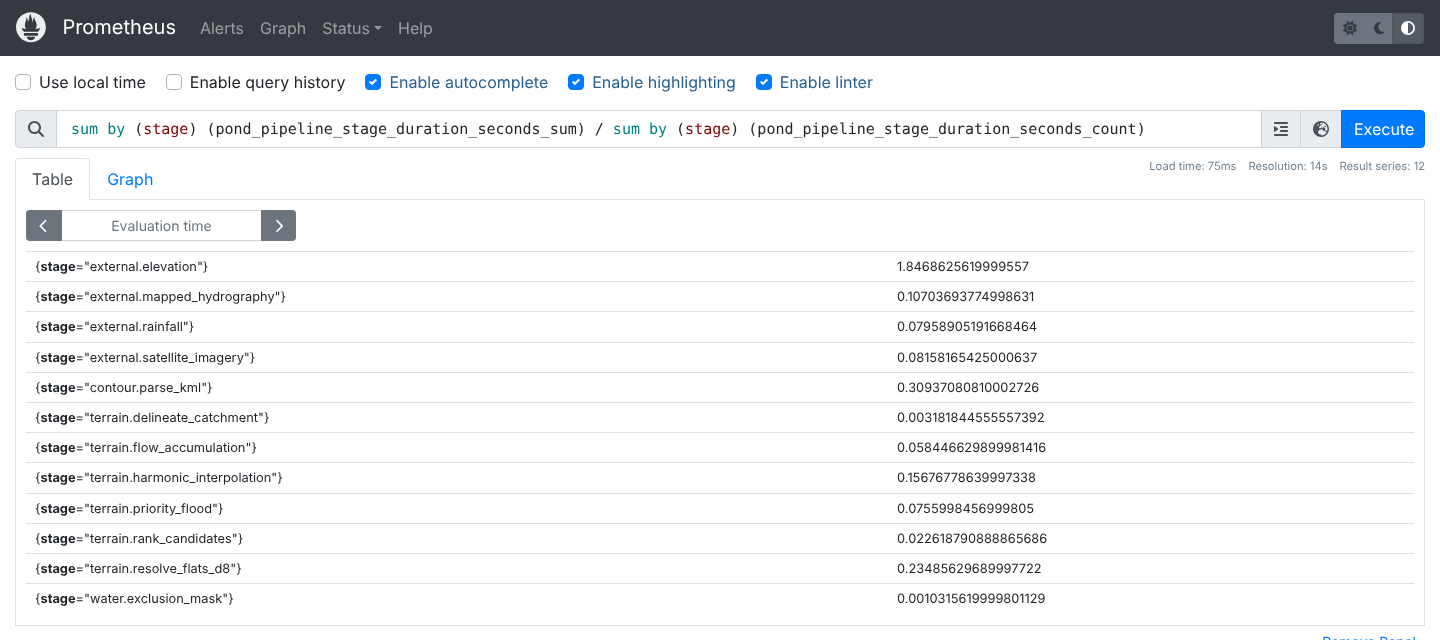
\includegraphics[width=\linewidth]{figures/f7_prom_stages.png}
\caption{Average time per pipeline stage from the \texttt{pond.pipeline.stage.duration} histogram. KML parsing (0.32 s) and flat resolution + D8 (0.24 s) dominate; catchment delineation is about 3 ms. External elevation (1.8 s) appears only in the failing live workflow.}\end{figure}

\begin{figure}[H]\centering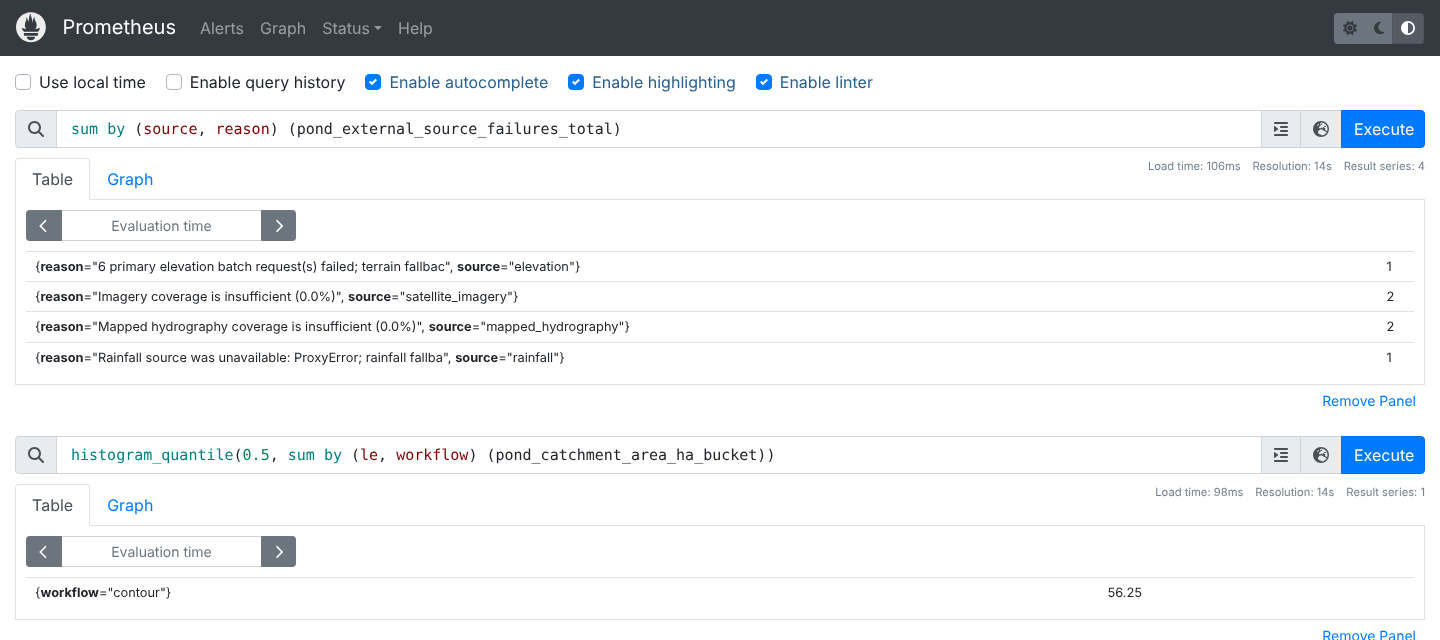
\includegraphics[width=\linewidth]{figures/f8_prom_failures.png}
\caption{Top: \texttt{pond.external\_source.failures} by source and reason (satellite imagery 2, mapped hydrography 2, rainfall 1, elevation 1). Bottom: median catchment area estimated from the histogram buckets (56 ha). Prometheus interpolates inside the 50--75 ha bucket; the exact values are in the traces.}\end{figure}

\begin{figure}[H]\centering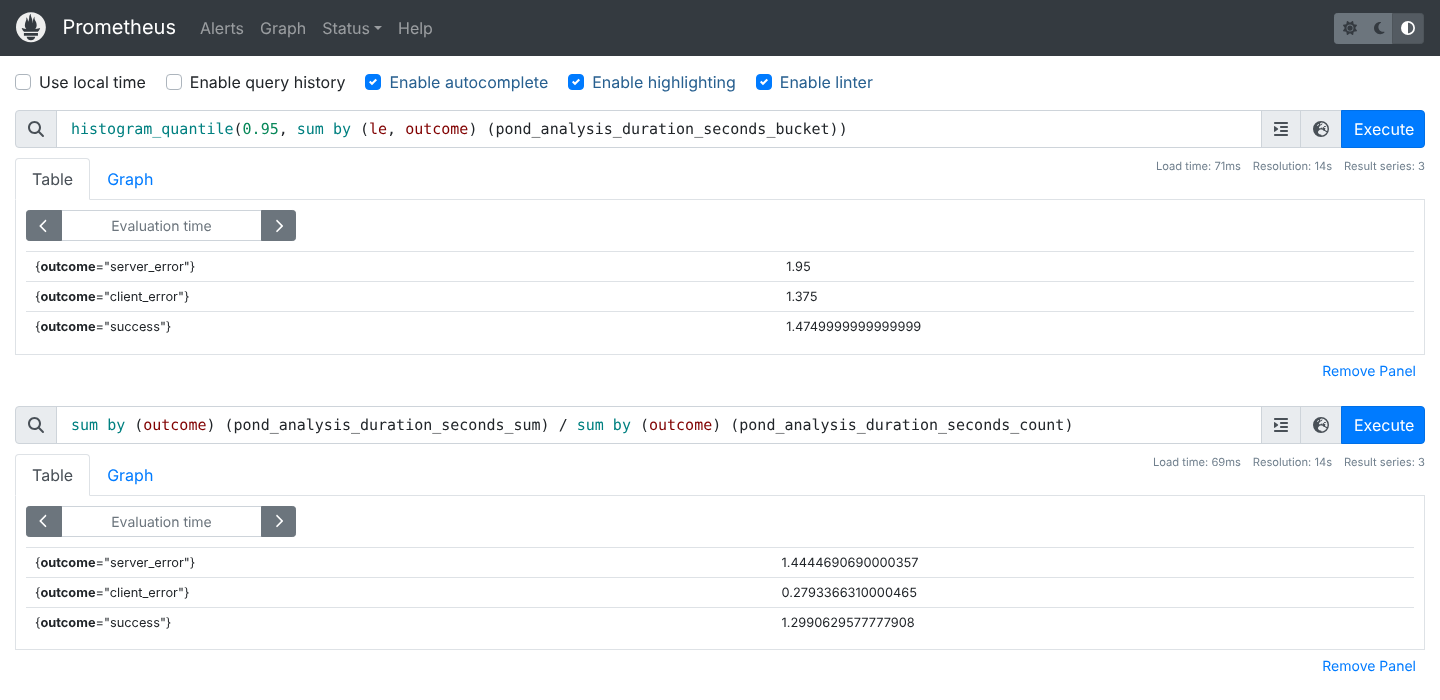
\includegraphics[width=\linewidth]{figures/f9_prom_latency.png}
\caption{Latency of analysis requests: p95 from the histogram (success 1.47 s, client error 1.38 s, server error 1.95 s) and mean duration per outcome (success 1.30 s). The client-error p95 is high because a river-point request is rejected only \emph{after} terrain analysis, while missing-file errors take milliseconds.}\end{figure}

\begin{figure}[H]\centering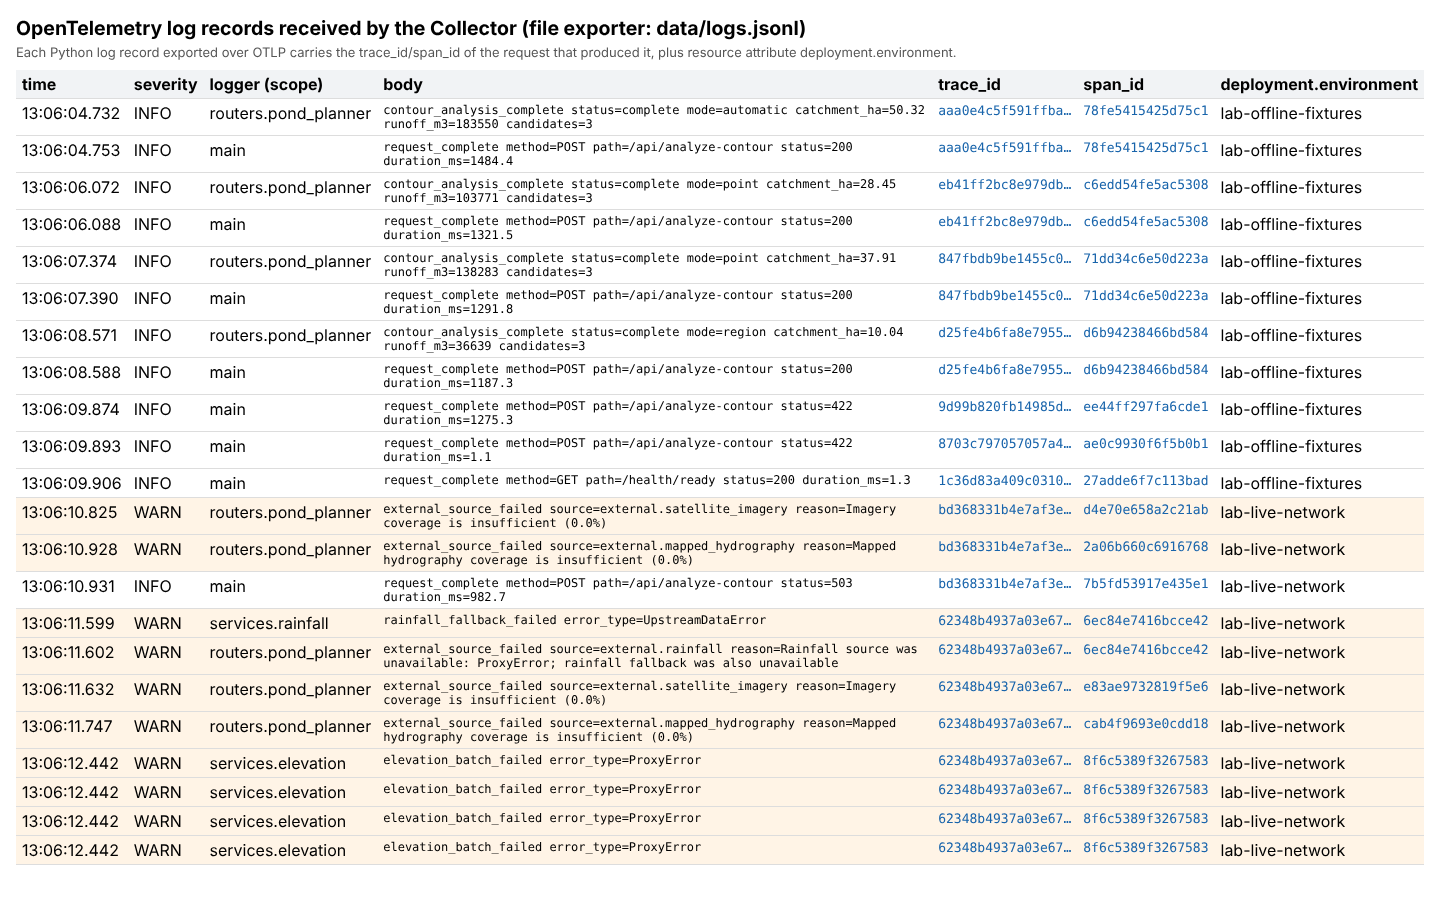
\includegraphics[width=\linewidth]{figures/f10_otlp_logs.png}
\caption{OTLP log records received by the Collector (file exporter). Each record has severity, logger, message, \textbf{trace\_id/span\_id} and \texttt{deployment.environment}. Successful analyses log mode, catchment and runoff; WARN rows record which external source failed and why. Any row can be matched to its Jaeger trace through the trace id.}\end{figure}

\begin{figure}[H]\centering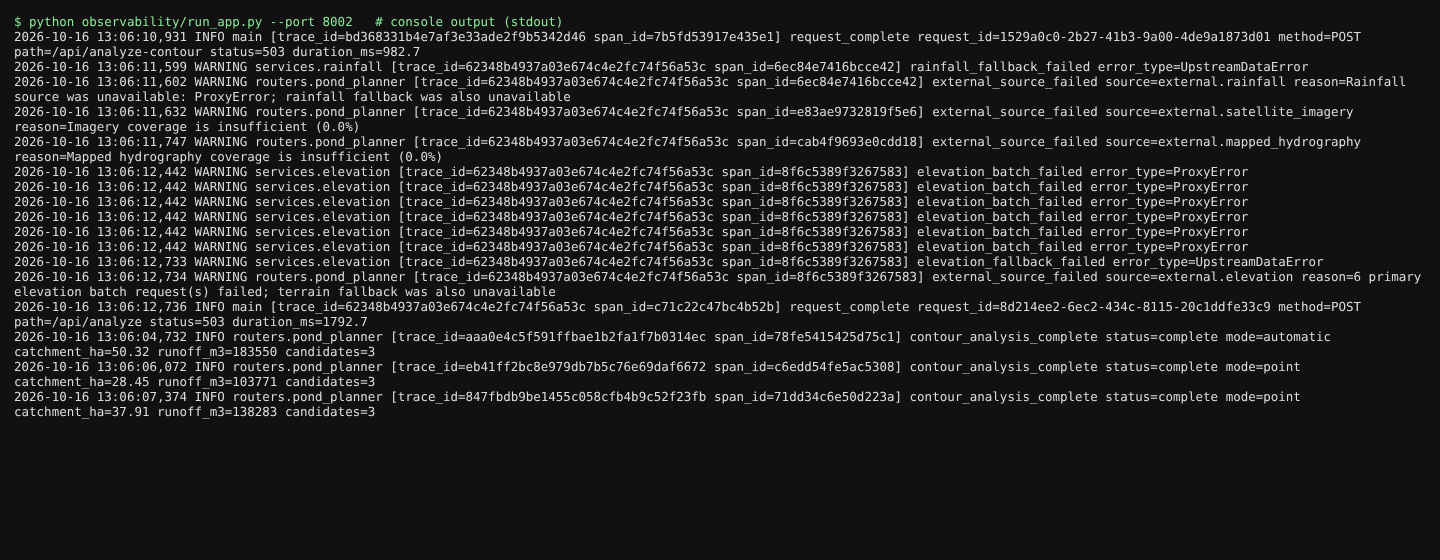
\includegraphics[width=\linewidth]{figures/f11_console_logs.png}
\caption{Application console output with trace correlation. All WARN lines of the failing live request share trace id \texttt{62348b49…}, the same trace as in the live-failure trace figure, so a developer can jump from a log line straight to the full trace.}\end{figure}

\section{Understanding of the collected data}
\textbf{Traces answer ``what happened in this one request, and where did the time go?''}
\begin{itemize}
\item The success trace shows external fetches overlapping in time, which proves the \texttt{asyncio.gather} concurrency described in my design.
\item Pure algorithm time is about 0.9~s of the 1.3--1.5~s request. The rest is reading the 6.7~MB upload and serialising the large JSON response (contours and catchment polygon).
\item \textbf{A finding from tracing:} there is a gap of about 0.37~s before the external spans start, and \texttt{contour.parse\_kml} appears again later. The route parses the KML once to get the map centre and the analyser parses it a second time. Passing the already-parsed dataset to the analyser would save about 0.3~s (roughly 25\%) per request. I would not have noticed this without the waterfall view.
\end{itemize}

\textbf{Metrics answer ``how is the service behaving over time?''} Request counts by status give the error rate. The duration histograms give p95 latency for a service-level objective, for example ``95\% of contour analyses under 3~s''. The failure counter shows which dependency is unreliable. The catchment and runoff histograms monitor the \emph{scientific output} distribution, so a sudden shift (e.g.\ all catchments becoming tiny) would reveal a data or code regression even when HTTP status codes are all 200. Metrics are cheap aggregates, so they can be kept for long periods and used for alerts, whereas traces show individual examples.

\textbf{Logs answer ``what exactly was the message?''} They hold human-readable detail (failure reasons, result summaries). Because every log carries the trace id, a WARN line in the console leads straight to the full trace in Jaeger, and a slow trace leads back to its logs.

\textbf{How this helps my application:}
\begin{itemize}
\item \textbf{Monitoring:} alert on a rising 5xx rate or rising \texttt{pond.external\_source.failures}. My app depends on four public data services, which is exactly where earlier demo failures came from.
\item \textbf{Debugging:} a 503 trace immediately names the failing source and the number of retries, instead of only ``analysis failed''.
\item \textbf{Analysis and optimisation:} stage timings show where to optimise (KML parsing, D8). Rate-limit hits (429) show when the per-minute limit is too strict for a demo.
\end{itemize}

\section{Limitations}
\begin{itemize}
\item The demonstration ran on my lab machine, not on the allotted college system. That system cannot install packages from PyPI and exposes only one web port, so running the Collector, Jaeger and Prometheus there was not attempted. The code is already in the repository and is switched on with \texttt{OTEL\_ENABLED=true} plus a Collector endpoint.
\item Success-path external data came from local fixtures (Section~2.4), so those three external spans measure fixture time, not network time. The failure-path spans are real network failures.
\item Jaeger used in-memory storage and every trace was sampled (100\%). Production use would need persistent storage and a sampling policy.
\item No Grafana dashboard was built; the Prometheus UI was used for queries.
\end{itemize}
\end{document}
